\chapter{Übersicht}
Diagramm \ref{design:dia:modules} gibt einen groben Überblick über alle Komponenten.
Das Programm teilt sich in zwei Hauptabschnitte: dem CrawlerModule (Python) und dem Server/Client (Java).


Das CrawlerModule dient als Backend. Hier werden die Seiten gecrawlt, Metadaten ausgelesen, gefiltert und 
schließlich ins Archiv und in die Datenbank geschrieben. Für den Java-Server wird ein Javadapter zur 
Verfügung gestellt, der es erlaubt, bestimmte Versionsstände auszuchecken, Dateien gegen gemeinsame
Zugriffe zu sperren und hinzugefügte Daten zu committen.


Der Java-Server und die Clients dienen als Frontend. Über eine Java-API können sich
Benutzer beim Server registrieren. Damit können folgende Abfragen an das Archiv gestellt werden:
Metadaten aus der Datenbank, Dateien aus dem Archiv sowie Datenelemente aus den begleiteten XML-Dateien.
Es können auch neue Dateien und XML-Elemente hinzugefügt werden.
Der serverinterne Notifier führt in regelmäßigen Abständen Abfragen auf die Datenbank nach neuen
Commits durch, welche dann an angemeldete Clients versendet werden, falls diese angemeldete Observer haben.

\begin{figure}
	\centering
	\label{design:dia:modules}
	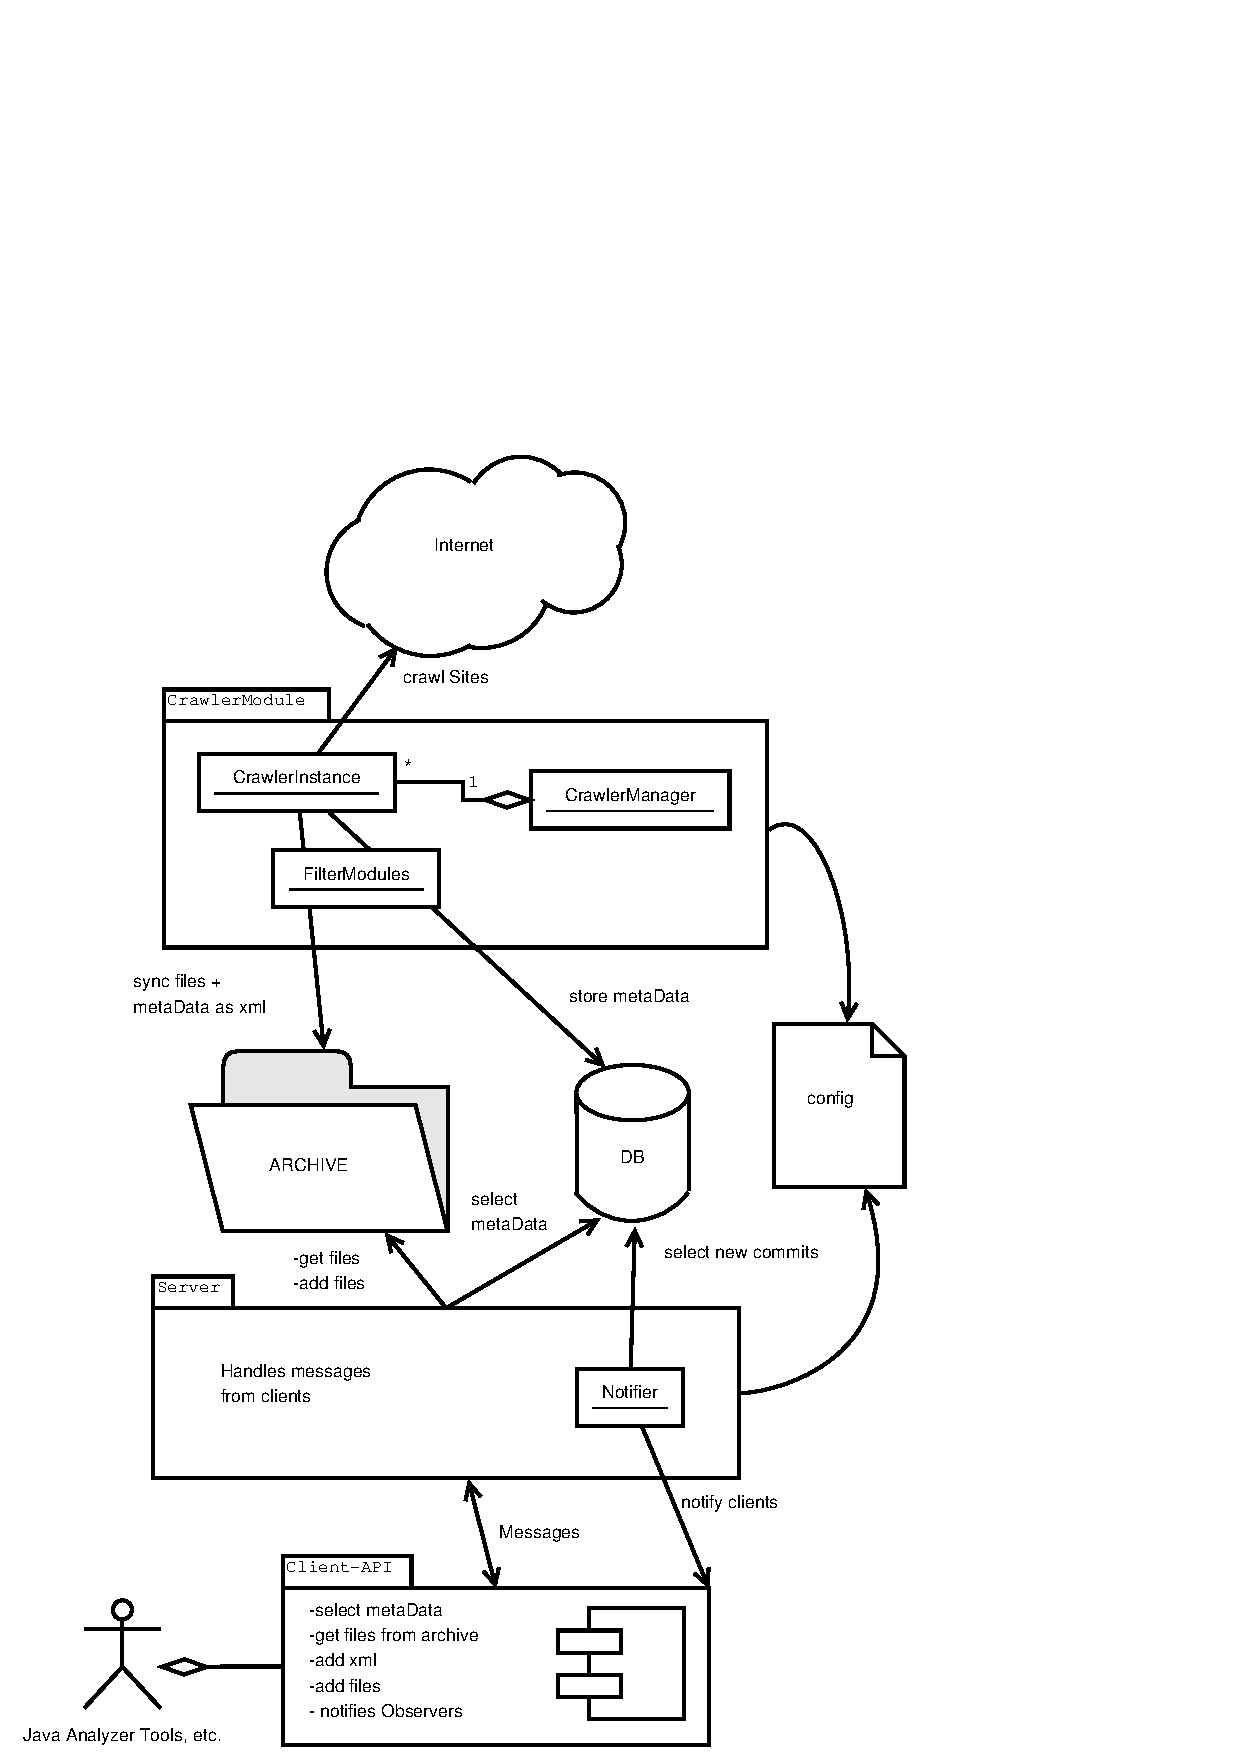
\includegraphics[height=\textheight]{design/components.pdf}
	\caption{Diagramm: Grundlegendes Design}
\end{figure}
